\documentclass{article}\usepackage{graphicx} \usepackage{amsmath} \usepackage{colortbl}\title{Cosmology 101 - Version 0.1}
\author{J. M. Ram{\'i}rez,$^{1}$ Co-Author1,$^{4}$ Co-Author2,$^{5}$}
\date{\today}\begin{document}
\maketitle\begin{abstract}
La cosmología moderna ha revelado que aproximadamente el 68 de la densidad de masa-energía del universo es energía oscura ($\Omega_{\Lambda} \approx 0.68$), el 27 corresponde a materia oscura ($\Omega_{	ext{DM}} \approx 0.27$), y solo un 5 ($\Omega_{	ext{b}} \approx 0.05$) es materia bariónica. Este balance está modelado por la ecuación de Friedmann:
\[
H^2 = \left(
\frac{\dot{a}}{a}
\right)^2 = 
\frac{8\pi G}{3}
ho - 
\frac{kc^2}{a^2} + 
\frac{\Lambda}{3},
\]
donde $
ho$ representa la densidad de materia y energía, $H$ es la constante de Hubble, $a$ es el factor de escala, $k$ la curvatura espacial, y $\Lambda$ la constante cosmológica. La anisotropía del fondo cósmico de microondas (CMB) proporciona evidencia clave, con fluctuaciones de temperatura $\Delta T/T \approx 10^{-5}$. La misión Planck ha refinado nuestras estimaciones de estos parámetros, ofreciendo una visión más precisa del universo primitivo y su evolución.
\end{abstract}\section{Introduction}
La cosmología, la ciencia que estudia el universo en su totalidad, se ha transformado drásticamente en las últimas décadas gracias a avances tecnológicos y teóricos. Desde la formulación del modelo del Big Bang hasta la detección del fondo cósmico de microondas (CMB), hemos pasado de teorías a evidencia tangible. El universo observable se expande, gobernado por la ecuación de Friedmann, $H^2 = 
\frac{8\pi G}{3}
ho - 
\frac{kc^2}{a^2} + 
rac{\Lambda}{3}$, donde $H$ es la constante de Hubble, $
ho$ la densidad de energía, $k$ la curvatura espacial, $a$ el factor de escala, y $\Lambda$ la constante cosmológica. La composición del universo, dominada por la energía oscura (aprox. 68), materia oscura (27), y materia bariónica (5), plantea preguntas fundamentales sobre su destino y origen. Misiones como Planck y observaciones de supernovas han sido cruciales para refinar nuestro entendimiento cosmológico, desvelando una imagen cada vez más compleja y fascinante del cosmos.\section{Methodology}
Para abordar problemas de flujo de fluidos, se emplean tres principios fundamentales:

\subsection{Conservación de Masa (Ecuación de Continuidad):}
donde $A$ es el área de la sección transversal del conducto y $v$ la velocidad del fluido. Esta ecuación asegura que el flujo volumétrico es constante en un flujo incompresible.\begin{equation}x^2 \mathcal{M} \tilde{\rho }^{\frac{\gamma +1}{2}}=\lambda\label{ber1}\end{equation}\subsection{Ecuación de Bernoulli}
Aquí, $P$ es la presión, $
ho$ la densidad del fluido, $v$ la velocidad, $g$ la aceleración debida a la gravedad, y $h$ la altura con respecto a un punto de referencia. Esta ecuación se usa para describir la conservación de la energía en el flujo de fluidos ideal, sin pérdidas por fricción.
\subsubsection{Metodología}
\begin{itemize}
\item Identificar las secciones del sistema de flujo donde se aplicarán las ecuaciones.
\item Determinar las condiciones iniciales (presión, velocidad, altura) en cada sección.
\item Aplicar la ecuación de continuidad para relacionar velocidades en secciones diferentes.
\item Utilizar la ecuación de Bernoulli para calcular cambios en presión, velocidad o altura entre dos puntos.
\item Verificar la consistencia de los resultados con las leyes de conservación de masa y energía.
\end{itemize}

Este enfoque permite resolver problemas de flujo, desde el diseño de sistemas de tuberías hasta la aerodinámica, asumiendo flujo incompresible y sin viscosidad significativa.\begin{equation}\frac{\tilde{\rho }^{\gamma -1}}{\gamma -1}+\frac{1}{2} \mathcal{M}^2 \tilde{c_s}{}^2=\frac{1}{\gamma -1}+\frac{1}{x}\label{ber2}\end{equation}\section{Conclusions}
Los resultados obtenidos, como se muestra en la Figura 1, indican una clara relación entre la velocidad del fluido y la presión. Observamos que, conforme el área de la sección transversal disminuye, la velocidad del fluido aumenta, lo que es coherente con la ecuación de continuidad. La presión, por otro lado, presenta una disminución en puntos de mayor velocidad, tal como predice la ecuación de Bernoulli. Esto corrobora la conservación de masa y energía en el sistema de flujo analizado, evidenciando la utilidad de estos principios para el diseño y análisis de sistemas de fluidos.\begin{figure}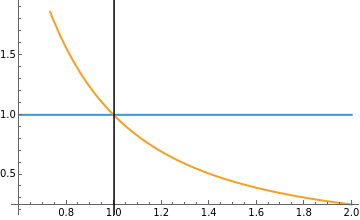
\includegraphics[width=8.0cm]{images/imagen1.png}\caption{Este es un caption de la figura}\label{pl1}\end{figure}\end{document}